
当我们接受了某些数据共享即将发生的事实,就必须接受对共享数据的同步。记住,在没有同步的情况下,对相同数据的任何并发访问都会导致数据竞争和未定义行为。

保护共享数据的最常用方法是使用互斥锁:

\begin{lstlisting}[style=styleCXX]
std::mutex m;
size_t count;// Guarded by m
… on the threads …
{
	std::lock_guard l(m);
	++count;
}
\end{lstlisting}

在这里,我们使用C++17模板类型推断来实现\texttt{std::lock\_guard}。在C++14中,必须指定模板类型实参。

使用互斥对象通常相当简单:访问共享数据的代码都应该位于临界区,也就是说,夹在锁定和解锁互斥对象的调用之间。互斥锁的实现带有正确的内存栅栏,以确保临界区中的代码不能被硬件或编译器移出临界区(编译器通常不会在锁操作中移动代码。不过,只要遵循内存栅栏的语义,理论上可以做这样的优化)。

这时候通常会问的是:“这个互斥锁的开销有多大?”然而,这个问题并没有很好地答案:对于特定的硬件和给定的互斥锁实现,当然可以给出绝对的答案,甚至以纳秒为单位,但是这个值有什么意义呢?这当然比没有互斥对象开销小得多,但没有互斥对象,程序结果就会不正确(而且有更简单的方法可以快速生成不正确的程序)。所以,“开销大”的定义只能与替代方案相比较,这自然引出了下一个问题,替代方案是什么?

最明显的替代方法是使计数原子化:

\begin{lstlisting}[style=styleCXX]
std::atomic<size_t> count;
… on the threads …
++count;
\end{lstlisting}

还必须考虑我们真正需要什么内存序来与计数上的操作相关联。如果稍后使用该计数,例如在数组中进行下标索引,那我们可能需要释放-获取序。但如果只是一个计数,只是要统计一些事件并报告数量,那我们不需要任何内存序限制:

\begin{lstlisting}[style=styleCXX]
std::atomic<size_t> count;
… on the threads …
count.fetch_add(1, std::memory_order_relaxed);
\end{lstlisting}

我们是否真的使用栅栏取决于硬件:在x86上,原子增量指令有“内置”的双向内存栅栏,自由序不会让它更快。尽管如此,为了可移植性和清晰性,指定代码真正需要的内存序仍然很重要:记住,写代码不是给解析代码的编译器看的,而是给需要阅读代码的其他开发者看的。

具有原子增量的程序没有锁,也不需要任何锁。然而,它依赖于特定的硬件能力:处理器有一个原子增量指令,这类指令的集合相当小。如果需要一个没有原子指令的操作,该怎么办?举个例子:在C++中,没有原子乘法(我不知道任何硬件有这样的能力。当然,在x86、ARM或其他任何通用CPU架构上都找不到)。

幸运的是,有一种“通用的”原子操作,可以用来构建任何读-改-写操作(困难程度不同)。这个操作称为\textbf{比较-交换},在C++中称为\texttt{compare\_exchange}。它有两个参数:第一个是原子变量的预期当前值,第二个是预期的新值。如果实际的当前值与期望值不匹配,则什么也不会发生,原子变量也不会发生更改。但是,如果当前值与期望值匹配,则需要的值将被写入原子变量。C++的\texttt{compare\_exchange}操作会返回true或false来指示写操作是否发生(如果发生则返回true)。如果变量与预期值不匹配,则在第一个参数中返回实际值。通过比较和交换,我们可以以以下方式实现原子增量操作:

\begin{lstlisting}[style=styleCXX]
std::atomic<size_t> count;
… on the threads …
size_t c = count.load(std::memory_order_relaxed);
while (!count.compare_exchange_strong(c, c + 1,
	std::memory_order_relaxed, std::memory_order_relaxed)) {}
\end{lstlisting}

首先,C++中操作的实际名称是\texttt{compare\_exchange\_strong}和\texttt{compare\_exchange\_weak}。不同的是,即使当前值和期望值匹配,弱版本有时也会返回false(在x86上,这没有区别,但在一些平台上,弱版本可以更快的进行)。其次,该操作接受两个(而不是一个内存序参数):第二个内存序应用于比较失败时(因此它只是操作的比较部分的内存顺序),第一个内存序应用于比较成功并发生写操作时。

来分析这个实现是如何工作的。首先,以原子的方式读取count的当前值\texttt{c}。当然,增量后是\texttt{c + 1},但我们不能直接将其赋值给count,因为在读取之后,在更新之前,另一个线程也可以将count赋值。因此,必须进行条件写入:如果count的当前值仍然是\texttt{c},则将其替换为所需的值\texttt{c + 1}。否则,用新的当前值更新\texttt{c} (\texttt{compare\_exchange\_strong}可以做到),然后再试一次。只有捕捉到原子变量,在上次读取它的时间和试图更新它之间没有变化时,循环才会退出。当然,有原子增量操作时,没有理由这样来增加计数。但这种方法可以推广到任何计算中:可以使用其他表达式,而不是\texttt{c + 1},程序将以同样的方式进行。

虽然这三个版本的代码都执行相同的操作,但它们之间有着根本性的区别,我们必须对此进行更详细的探讨。

\subsubsubsection{6.3.1\hspace{0.2cm}基于锁、无锁和无等待的程序}

第一个版本,使用互斥锁,是最容易理解的:一个线程可以在任何时候持有锁,因此线程可以在没有任何进一步的注意的情况下增加计数。当锁被释放,另一个线程可以获取它并增加计数,依此类推。在任何时候,最多只能有一个线程持有锁并进行任何操作,所有需要访问的剩余线程都在等待该锁。但是,即使拥有锁的线程也不能保证可以正常运行。如果它需要在完成它的任务之前访问另一个共享变量,那么可能需要等待由其他线程持有的锁。这是常见的基于锁的程序,通常不是最快的,但最容易理解。

第二个程序呈现了一个非常不同的场景:到达原子增量操作的线程都会毫不延迟地执行它。当然,硬件本身必须锁定对共享数据的访问,以确保操作的原子性(这是通过一次将对整个缓存线的独占访问授予一个处理器来实现的)。从开发者的角度来看,这种独占访问表明其本身会增加执行原子操作所需的时间。然而,代码本身没有等待,没有尝试和再尝试。这种程序称为\textbf{无等待}程序。在一个无等待的程序中,所有线程都能正常运行。也就是说,在任何时候都在执行操作(尽管线程之间为了访问同一个共享变量而发生争用,有些操作可能会花费更长的时间)。无等待的实现通常只适用于非常简单的操作(例如增加计数),但只要有这种实现,甚至会比基于锁的实现更简单。

要理解最后一个程序的行为需要付出更多的努力。这里没有锁,但有一个循环重复了未知的次数。这里的实现类似于锁,任何等待锁的线程也会困在一个类似的循环中,不停的尝试获得锁。但是,有一个关键的区别:在基于锁的程序中,当一个线程获取锁失败,必须再次尝试时,可以推断其他线程拥有锁。我们不能确定线程是否会很快释放锁,或者其工作有任何进展(例如,它可能正在等待用户输入一些东西)。在基于比较-交换的程序中,我们的线程无法更新共享计数的唯一原因是其他线程对先其进行了更新。因此,在所有试图同时增加计数的线程中,至少有一个是成功的。这种程序称为\textbf{无锁}程序。

我们已经了解了三种主要类型的并发程序的例子:

\begin{itemize}
\item 在无等待的程序中,每个线程都在执行它需要的操作,并且总是朝着最终目标前进。不需要等待访问,也不需要重做任何工作。

\item 在无锁程序中,多个线程可能试图更新相同的共享数据,但只有一个会成功。其余的将不得不放弃它们基于原始值所做的工作,读取更新后的值,并再次进行计算。但至少有一个线程总是保证提交它的工作,而不必重做。因此,尽管不一定是全速前进,但整个程序是在前进的。

\item 最后,在基于锁的程序中,线程持有使其能够访问共享数据的锁。但是,仅仅因为持有锁并不意味着会对这些数据做什么。因此,当并发访问发生时,最多只有一个线程在有进展,但这也无法保证。
\end{itemize}

理论上讲,这三个程序之间的区别是显而易见的。但是,我敢打赌,每个读者都想知道的答案:哪个版本更快?我们可以在谷歌基准测试中运行每个版本的代码。例如,下面是基于锁的版本:

\hspace*{\fill} \\ %插入空行
\noindent
\textbf{01\_sharing\_incr\_mbm.C}
\begin{lstlisting}[style=styleCXX]
std::mutex m;
size_t count = 0;
void BM_lock(benchmark::State& state) {
	if (state.thread_index == 0) count = 0;
	for (auto _ : state) {
		std::lock_guard l(m);
		++count;
	}
}
BENCHMARK(BM_lock)->Threads(2)->UseRealTime();
\end{lstlisting}

必须在线程之间共享的变量在全局作用域中声明。初始设置(如果有的话)可以限制为一个线程。其他基准也类似,只有测试的代码发生了变化。下面是结果:

%\hspace*{\fill} \\ %插入空行
\begin{center}
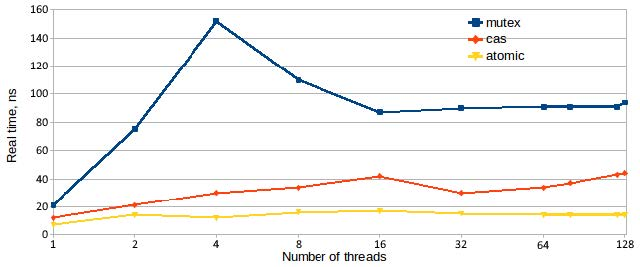
\includegraphics[width=0.9\textwidth]{content/2/chapter6/images/1.jpg}\\
图6.1 - 共享计数增量的性能:基于互斥锁、无锁(比较-交换,或CAS)和无等待(原子)
\end{center}

这里唯一想不到的结果是,基于锁的版本的性能非常差。然而,这只是一个数据点,而不是全部。特别是,虽然所有互斥对象都是锁,但并不是所有的锁都是互斥对象。我们可以尝试提出一种更有效的锁实现(至少,以满足我们的需求)。

\subsubsubsection{6.3.2\hspace{0.2cm}不同的问题使用不同的锁}

我们已经看到,标准的C++互斥锁在保护对共享变量的访问时性能非常差,特别是当有很多线程试图在同一时间修改这个变量时(如果所有线程都在读取这个变量,我们根本不需要保护它,并发只读访问不会导致任何数据竞争)。但是,锁的效率低下是因为它的实现,还是因为锁的本质本身存在问题?根据前一章的了解,我们可以预期锁的效率都比原子递增计数器低,这是因为基于锁的方案使用两个共享变量(锁和计数),而原子计数器只使用一个共享变量。然而,操作系统提供的互斥对象对于锁定非常短的操作(比如计数增量)通常不是特别有效。

对于这种情况,最简单也是最有效的锁是自旋锁。自旋锁的思想是:锁本身只是一个可以有两个值的标志,比如0和1。如果flag值为0,表示不锁定。任何看到这个值的线程都可以将标志设置为1并继续。当然,读取标志并将其设置为1的整个操作必须是原子操作。任何看到值为1的线程都必须等待,直到该值变回0,以表明锁可用。最后,当一个将标志从0更改为1的线程准备释放锁时,它将把值更改回0。

这个锁的实现代码如下:

\begin{lstlisting}[style=styleCXX]
class Spinlock {
	public:
	void lock() {
		while (flag_.exchange(1, std::memory_order_acquire)) {}
	}
	void unlock() { flag_.store(0, std::memory_order_release); }
	private:
	std::atomic<unsigned int> flag_;
};
\end{lstlisting}

代码中,只展示了锁定和解锁函数。类还需要默认构造函数(原子整数在其自己的默认构造函数中初始化为0),以及使其不可复制的声明。

注意,锁定标志不使用条件交换,而总是将1写入标志。原因是,如果标志的原始值是0,交换操作将它设置为1并返回0(循环结束),这就是我们想要的。但是如果原来的值是1,它就被1代替,也就是不改变。

另外,注意两个内存栅栏:锁定伴随着获取栅栏,解锁伴随着打开栅栏。这些栅栏一起划分了临界区,并确保在\texttt{lock()}和\texttt{unlock()}调用之间的代码都留在那里。

您可能希望看到这个锁与标准互斥锁的基准比较,但是我们不打算展示:这个自旋锁的性能非常糟糕。为了使它有用,需要一些优化。

首先,请注意,如果标志的值是1,实际上不需要用1替换它,我们可以不去管它。为什么这很重要?交换是一个读-改-写操作。即使它将旧的值更改为相同的值,也需要独占访问包含该标志的缓存行,我们不需要独占访问来读取该标志。这在以下场景中很重要:一个锁锁住了,拥有锁的线程没有更改它(正在忙着做它的工作),但是其他线程都在检查锁并等待锁的值更改为0。如果它们不尝试写入标志,那么缓存行就需要在CPU之间切换:它们都有相同的内存副本在缓存中,并且这个副本是当前的,不需要发送数据到其他地方。只有当其中一个线程实际改变了值时,硬件才需要将内存中的新内容发送给所有的CPU。下面是我们刚刚描述的优化,以代码的形式完成:

\begin{lstlisting}[style=styleCXX]
class Spinlock {
	void lock() {
		while (flag_.load(std::memory_order_relaxed) ||
		flag_.exchange(1, std::memory_order_acquire)) {}
	}
}
\end{lstlisting}

这里做的优化是,首先读取该标志,直到看到0,然后将其与1交换。如果另一个线程先获得了锁,那么在进行检查和交换之间,这个值可以变成1。另外,在预检查标志时,我们根本不关心内存栅栏,因为最终的决定性检查会使用交换和内存栅栏来完成。

即使进行了这种优化,锁的性能仍然很差。原因与操作系统倾向于优先处理线程的方式有关。当一个线程正在做一些有用的事情,那么将会获得更多的CPU时间。不幸的是,在我们的例子中,计算量最大的线程是在等待标志改变的同时,查询获得标志线程的状态。这可能会导致一种不希望出现的情况,即一个线程试图获得锁并将CPU分配给它,而另一个线程希望释放锁,但在一段时间内没有调度执行。解决方案是等待的线程在多次尝试后放弃CPU,这样其他线程就可以运行,并且可以完成它自己的工作并释放锁。

有几种方法可以让线程释放对CPU的控制,大多数都是通过系统函数调用完成的,没有一个通用的最好的方法。在Linux上,通过调用\texttt{nanosleep()}在很短的一段时间内(1纳秒)调用\texttt{sleep},可能会产生最好的结果,通常比调用\texttt{sched\_yield()}更好,\texttt{sched\_yield()}是另一个提供CPU访问的系统函数。与硬件指令相比,所有的系统调用都开销很大,所以最好不要过于频繁地调用。当尝试几次获取锁,然后将CPU交给另一个线程,然后再尝试时,就达到了最佳的平衡:

\hspace*{\fill} \\ %插入空行
\noindent
\textbf{01c\_spinlock\_count.C}
\begin{lstlisting}[style=styleCXX]
class Spinlock {
	void lock() {
		for (int i=0; flag_.load(std::memory_order_relaxed) ||
		flag_.exchange(1, std::memory_order_acquire); ++i) {
			if (i == 8) {
				lock_sleep();
				i = 0;
			}
		}
	}
	void lock_sleep() {
		static const timespec ns = { 0, 1 }; // 1 nanosecond
		nanosleep(&ns, NULL);
	}
}
\end{lstlisting}

在释放CPU之前,获取锁的最佳尝试次数取决于硬件和线程数,但一般来说,8到16之间的值比较合适。

现在,我们已经准备好进行第二轮的基准测试了,结果如下:

%\hspace*{\fill} \\ %插入空行
\begin{center}
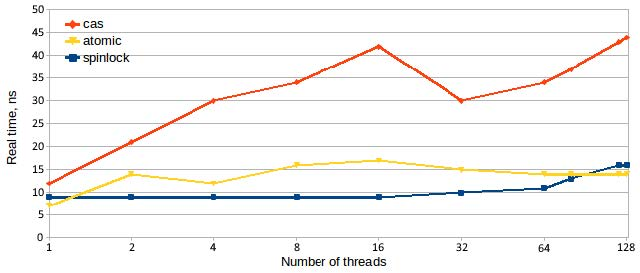
\includegraphics[width=0.9\textwidth]{content/2/chapter6/images/2.jpg}\\
图6.2 - 共享计数增量的性能:基于自旋锁、无锁(比较-交换,或CAS)和无等待(原子)
\end{center}

自旋锁已经做得很好了:它的性能明显优于比较-交换实现,并可以与无等待操作进行竞争。这里会有两个问题:首先,如果自旋锁的速度快得多,为什么不是所有锁都使用自旋锁?其次,如果自旋锁这么好,为什么我们甚至还需要原子操作(当然,除了锁实现的原子操作)?

第一个问题的答案可以归结为本节的标题:不同的问题使用不同的锁。自旋锁的缺点是等待的线程不断地使用CPU或“忙等待”。另一方面,等待系统互斥的线程大部分是空闲的(休眠)。如果需要等待几个周期,即增量操作的持续时间,那么忙碌等待也不错:它比让线程进入睡眠状态要快得多。另一方面,如果锁定的计算包含多个指令,那么等待自旋锁的线程将浪费大量CPU时间,并剥夺其他工作线程访问它们所需的硬件资源的机会。总的来说,C++的互斥量(\texttt{std::mutex})或OS的互斥量通常会进行平衡:锁定一条指令的效率有点低,锁定一个需要几十纳秒的计算是可以的,如果需要保持锁很长时间(长是相对的,处理器很快,所以1毫秒是非常长的),这就打败了另一种选择。现在,我们讨论了极端性能(以及极端实现性能的努力),因此大多数HPC开发者要么实现自己的快速锁来保护短计算,要么使用现成的库。

第二个问题,“锁还有其他的缺点吗?”让我们带着这个问题进入下一节。

\subsubsubsection{6.3.3\hspace{0.2cm}基于锁的和无锁的区别}

在讨论无锁编程的好处时,第一个点通常是“更快”。但这并不一定是真的,如果针对特定的任务进行优化,锁的实现可以非常高效。但是,基于锁的方法还有其他缺点,不过这些	缺点不依赖于实现。

最头痛的是可能出现死锁。当程序使用多个锁时,就会发生死锁,比如lock1和lock2。线程A拥有lock1,需要获取lock2。线程B已经拥有了lock2,需要获取lock1。两个线程都不能继续,而且都将永远等待,因为唯一可以释放它们所需锁的线程被锁阻塞了。

如果同时获得两个锁,如果总是以相同的顺序获得锁,就可以避免死锁。C++有一个用于此目的的函数\texttt{std::lock()}。但通常不能同时获得锁,当线程A获得lock1时,无法知道我们也需要lock2,因为该信息隐藏在由lock1保护的数据中。我们将在下一章讨论并发数据结构时看到一些例子。

如果不能获取多个锁,也许解决方案会尝试获取它们。然后,若不能获得所有的锁,那么我们释放已经持有的锁,以便其他线程可以获得它们?在我们的例子中,线程A持有lock1,它也会尝试获得lock2,但不会阻塞:大多数锁都有\texttt{try\_lock()},要么获得锁,要么返回false。后一种情况下,线程A释放lock1并试图再次锁定它们。这可能行得通,特别是在一个简单的测试中。但它也有自己的危险:当两个线程不断地互相传递锁时,就会出现活锁:线程A有lock1,但没有lock2,线程B有lock2,放弃了它,得到了lock1,现在它不能再得到lock2了,因为线程A拥有了lock2。有一些算法可以获取多个锁,从而保证最终成功。不幸的是,这可能要经过很长一段时间,并且这些算法也相当复杂。

解决多个锁的问题是互斥对象不能组合,不好将两个或多个锁组合成一个。

即使没有活锁和死锁的危险,基于锁的程序也会遇到其他问题。其中较为频繁且难以诊断的一种称为协同。它可以在多个锁中发生,也可以只在一个锁中发生。协同看起来是这样的:假设我们有一个被锁保护的计算。线程A目前拥有这个锁,并且正在对共享数据进行操作,其他线程正在等待完成它们的那部分工作。然而,这项工作并不是一次性的:每个线程都有许多任务要做,每个任务的一部分需要独占访问共享数据。线程A完成一个任务,释放锁,然后快速切换到下一个任务,直到它再次需要锁。锁被释放了,任何其他线程都可以得到它,但其他线程没完全醒,而线程A在CPU上,而且没睡。因此,线程A再次获得锁,只是因为竞争对手还没有为它做好准备。线程A的任务像车队中的卡车一样快速执行,而在其他线程上什么也做不了。

然而,锁的另一个问题是,它们没有优先级的概念:持有锁的低优先级线程可以抢占任何需要相同锁的高优先级线程。因此,高优先级线程必须等待低优先级线程决定的时间,这种情况似乎与高优先级的概念完全不一致,这种情况有时称为优先级倒置。

既然我们已经理解了锁的问题并不局限于性能,那么让我们看看无锁程序在相同的复杂性下会有怎样的表现。首先,在无锁程序中,至少有一个线程不被阻塞:最坏的情况是,当所有线程同时执行比较-交换(CAS)操作,并且原子变量的期望与当前值相同时,其中一个线程将看到期望值(因为惟一可以更改的方法是通过CAS操作)。其他线程将放弃它们的计算结果,重新加载原子变量,并重复计算,但是在CAS上成功的线程可以移动到下一个任务,这避免了死锁的可能性。如果排除了死锁和避免死锁的尝试,我们也不必担心活锁。由于所有线程都在忙于计算通向原子操作(如CAS)的路径,高优先级线程更有可能首先到达那里并提交其结果,而低优先级线程更有可能使CAS失败,并不得不重做其工作。类似地,提交结果的一次成功并不会使“获胜”的线程比所有其他线程有任何优势:准备先尝试执行CAS的线程就是成功的线程。这自然就消除了协同的可能。

那么,无锁编程有什么不好呢?其有两个主要的缺点。第一个是其优点的反面,即使CAS尝试失败的线程也会保持忙碌。这解决了优先级问题,但代价很高:在高争用的情况下,大量的CPU时间被浪费在重复工作上。更糟糕的是,这些为访问单个原子变量而竞争的线程会从进行一些不相关计算的其他线程那里夺取CPU资源。

第二个缺点性质完全不同。虽然大多数并发程序都不容易编写或理解,但无锁程序的正确设计和实现非常困难。基于锁的程序只需要保证构成单个逻辑事务的操作集都在锁下执行。当存在多个逻辑事务时,例如(而不是所有)共享数据对几个不同的事务来说是公共的,这就更难了。这就是我们提出多锁问题的原因。尽管如此,推断基于锁的程序的正确性并不是那么困难:如果在代码中看到一段共享数据,就必须说明哪个锁保护该数据,并证明没有线程可以在不先获取该锁的情况下,访问该数据。如果不是这样,那么就会出现数据竞争。如果满足了这些需求,就不会出现数据竞争(尽管可能会出现死锁和其他问题)。

另一方面,无锁程序有无限多种数据同步方案。因为没有线程会暂停,所以我们必须说服自己,无论线程执行原子操作的顺序如何,结果都是正确的。此外,如果没有明确定义的临界区,就得担心内存序和程序中所有数据的可见性,而不仅仅是原子变量。我们必须问自己,有没有可能因为内存顺序要求不够严格,一个线程可以更改数据,而另一个线程可以看到它的旧版本?

解决复杂性问题的通常方法是模块化和封装。我们将复杂的代码收集到模块中,每个模块都有一个定义良好的接口和一组明确的需求和保证。主要关注实现各种并发算法的模块。不过本书会有一个不同的方向,本章的其余部分将专门讨论并发数据结构。




































